\chapter{Manufacturing of Planar Detectors}
The manufacturing process of a planar HPGe detector begins with a slice from a crystal boule that has been tested for quality and is know to be detector grade. Typical boules slices are solid discs that can range from a few millimeters up to several centimeters in thickness and 5+ centimeters in diameter. This large size allows for several detector samples to be cut from each slice so careful geometry considerations are important in order to minimize wasted material.
% INSTERT PICTURE OF DETECTOR SHAPE 2 WINGS AND 4 WITH DIMENSIONS


\subsection{Mechanical Processing}

\subsection{Chemical Processing}

\subsection{Amorphous Ge Deposition}

\begin{sidewaysfigure}
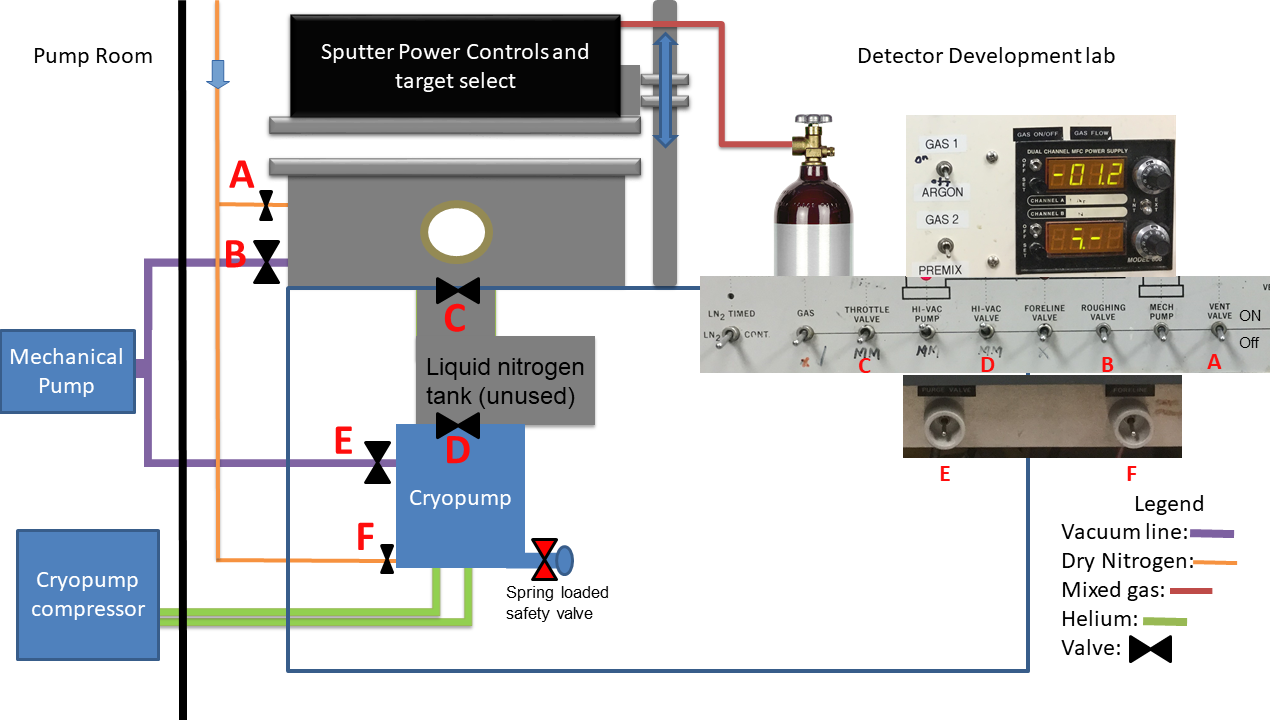
\includegraphics[width=\textwidth]{figures/sput-flow}
\caption{This is another example Figure, rotated to landscape orientation.}
\label{LandscapeFigure}
\end{sidewaysfigure}

\subsection{Aluminum Deposition}


\sunsection{Final Steps}
